%%%%%%%%%%%%%%%%%%%%%%%%%%%%%% Slide %%%%%%%%%%%%%%%%%%%%%%%%%%
\subsection{Figures}
%%%%%%%%%%%%%%%%%%%%%%%%%%%%
\begin{frame}[fragile,t]{Add Figures to Slides}
	\begin{itemize}
		\item Latex and beamer can use many different formats to make figures
		\begin{itemize}
			\item Ex: pdf, eps, png, jpeg, etc.
		\end{itemize}
\vspace{0.2in}
		\item \textbf{Aside:} recommend you save figures and graphs as vector graphics (eps, pdf, etc.) whenever possible
		\begin{itemize}
			\item Does not have the same issue with resolution and scaling as is the case with standard jpeg, png pictures
			\item Can save eps figures in Matlab and Python
		\end{itemize}
	\end{itemize}
\end{frame}

%%%%%%%%%%%%%%%%%%%%%%%%%%%%
\begin{frame}[fragile,t]{Add Figures to Slides}
	\begin{itemize}
		\item EPS file
		\begin{center}
			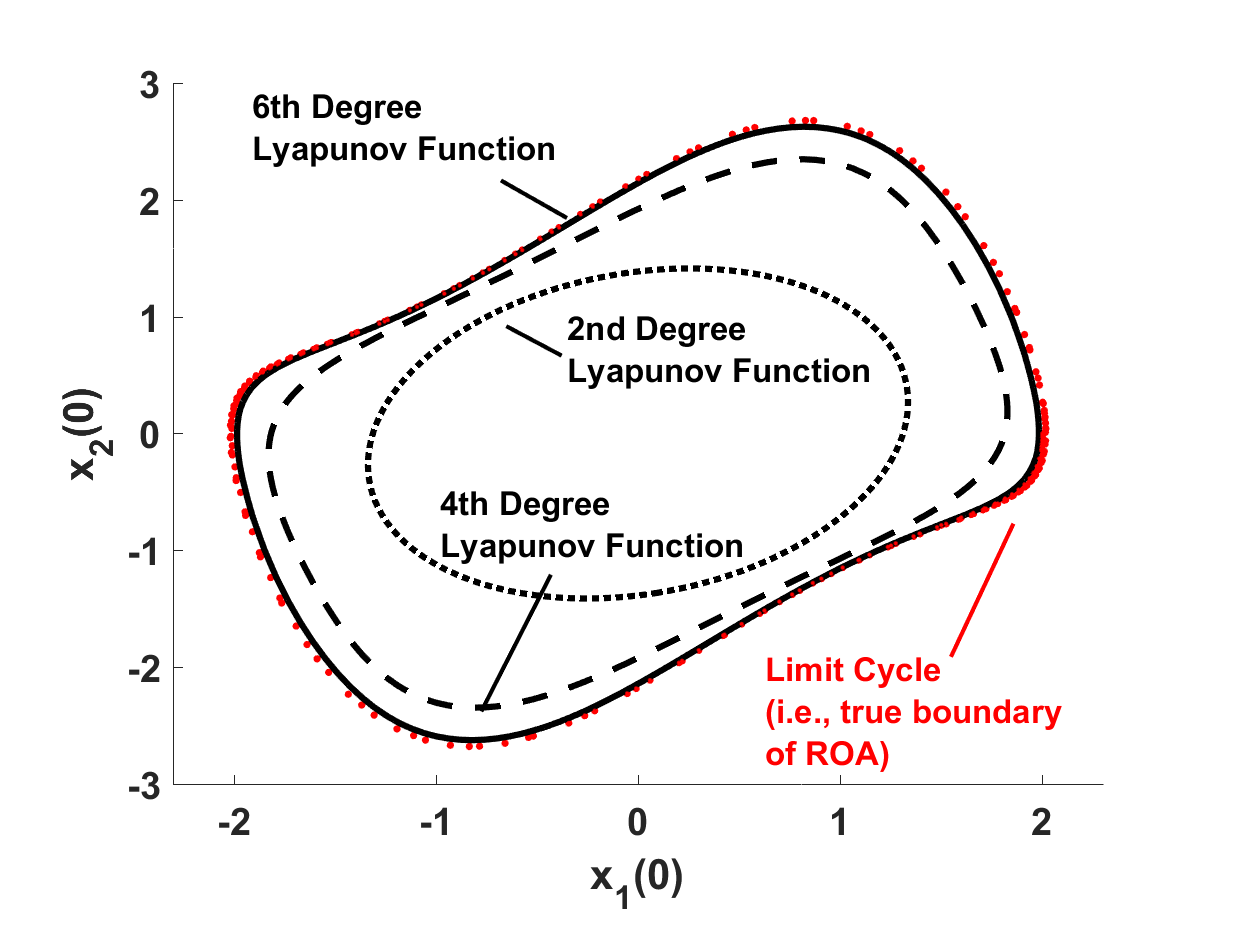
\includegraphics[width=0.85\columnwidth]{figures/my_figure.eps}
		\end{center}
	\end{itemize}
\end{frame}

%%%%%%%%%%%%%%%%%%%%%%%%%%%%
\begin{frame}[fragile,t]{Add Figures to Slides}
	\begin{itemize}
		\item PNG file (should look a little blurrier than the eps version)
		\begin{center}
			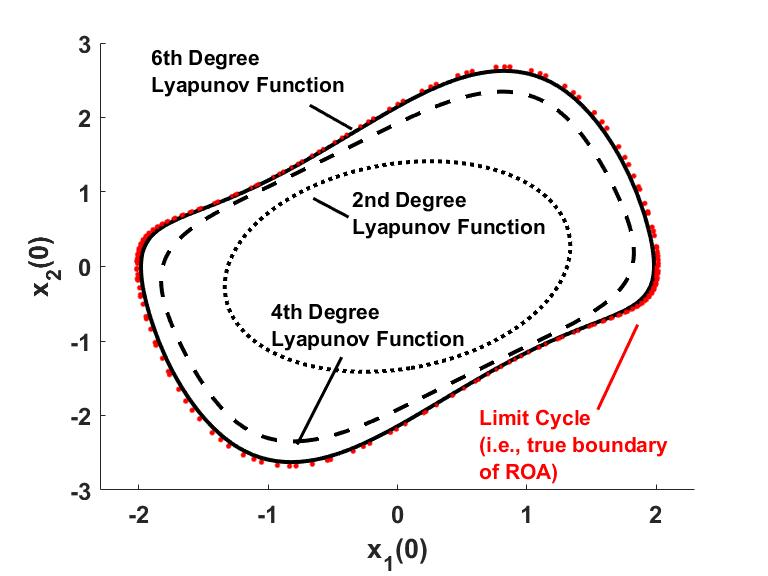
\includegraphics[width=0.85\columnwidth]{figures/my_figure.jpg}
		\end{center}
	\end{itemize}
\end{frame}


%%%%%%%%%%%%%%%%%%%%%%%%%%%%%% Slide %%%%%%%%%%%%%%%%%%%%%%%%%
%%%%%%%%%%%%%%%%%%%%%%%%%%%%
\begin{frame}[fragile,t]{Add Figures to Slides}
	\begin{itemize}
		\item Add a figure using the command
		\begin{verbatim}
			\includegraphics[picture size]{file location}
		\end{verbatim}
		\begin{itemize}
			\item \verb|[picture size]| - I use the \verb|\columnwidth| command to set width as a decimal $(0,1]$
			\begin{itemize}
				\item Ex: \verb|[width = 0.85\columnwidth]| - it scales the height of the figure to match the original aspect ratio
			\end{itemize}
			\item \verb|{file location}| - you need to match the file location and extension of the picture file
			\begin{itemize}
				\item The file location is relative to the main TeX file
				\item I typically save my figures in a subfolder labeled ``figures''
				\item Ex: \verb|{figures/my_figure.eps}|
			\end{itemize}
		\end{itemize}
	\end{itemize}
\end{frame}

%%%%%%%%%%%%%%%%%%%%%%%%%%%%
\begin{frame}[fragile,t]{Add Figures to Slides}
	\begin{itemize}
		\item Add a figure using the command
		\begin{verbatim}
			\includegraphics[picture size]{file location}
		\end{verbatim}
		\begin{itemize}
			\item \verb|[picture size]| - I use the \verb|\columnwidth| command to set width as a decimal $(0,1]$
			\begin{itemize}
				\item Ex: \verb|[width = 0.85\columnwidth]| - it scales the height of the figure to match the original aspect ratio
			\end{itemize}
			\item \verb|{file location}| - you need to match the file location and extension of the picture file
			\begin{itemize}
				\item The file location is relative to the main TeX file
				\item I typically save my figures in a subfolder labeled ``figures''
				\item Ex: \verb|{figures/my_figure.eps}|
			\end{itemize}
		\end{itemize}
		\item When appropriate, can center the figure (height and width) using
		{\small
		\begin{lstlisting}
\begin{center}
	\includegraphics[picture size]{file location}
\end{center}
		\end{lstlisting}
		}
	\end{itemize}
\end{frame}

%%%%%%%%%%%%%%%%%%%%%%%%%%%%
\begin{frame}[fragile,t]{Make a Figure}
	\begin{itemize}
		\item Here's the sample code to make the following figure
		{\tiny
		\begin{lstlisting}
\begin{center}
	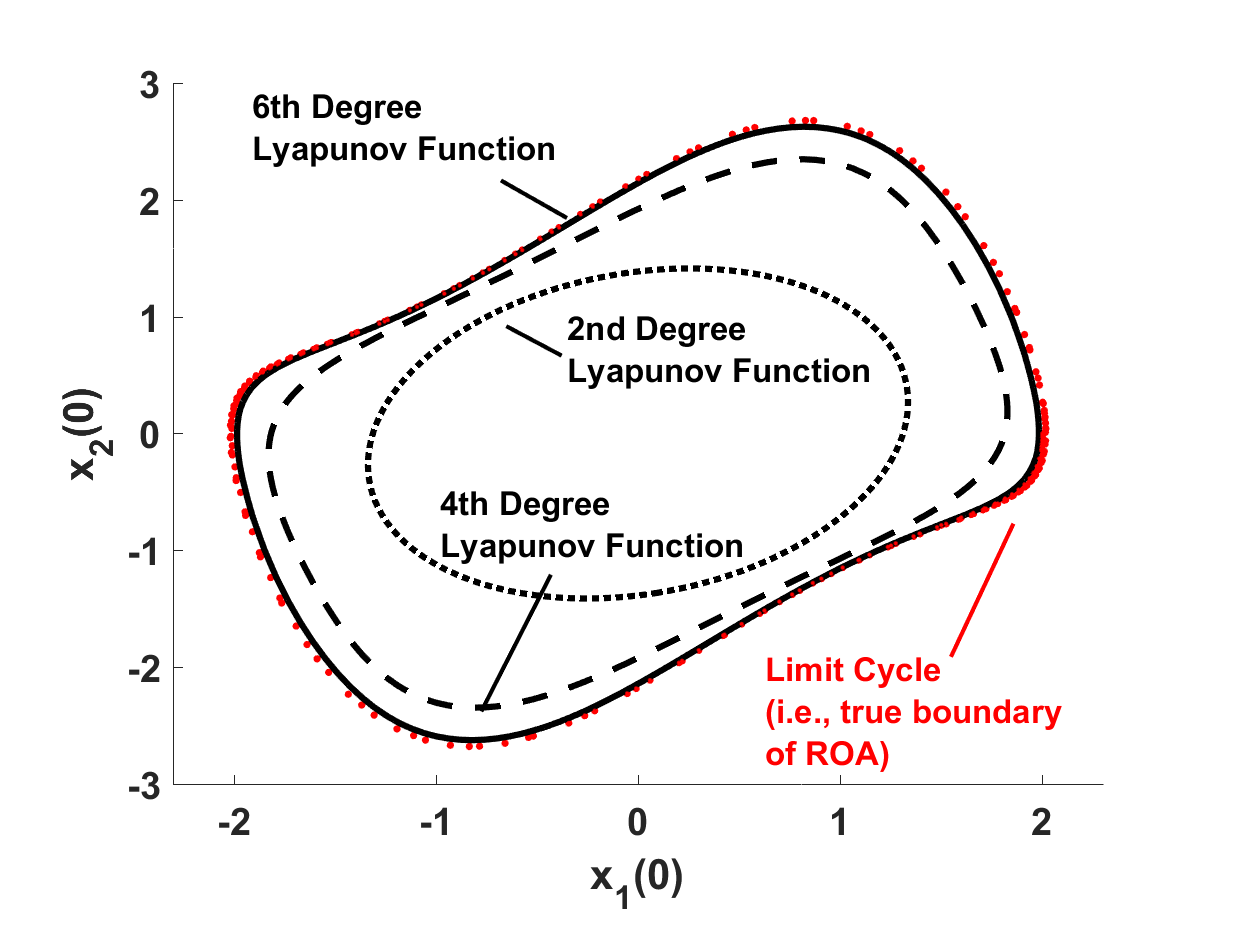
\includegraphics[width=0.65\columnwidth]{figures/my_figure.eps}
\end{center}
		\end{lstlisting}
		}
\vspace{-12pt} %removes white space between (opposite of positive values in vspace)
		\begin{center}
			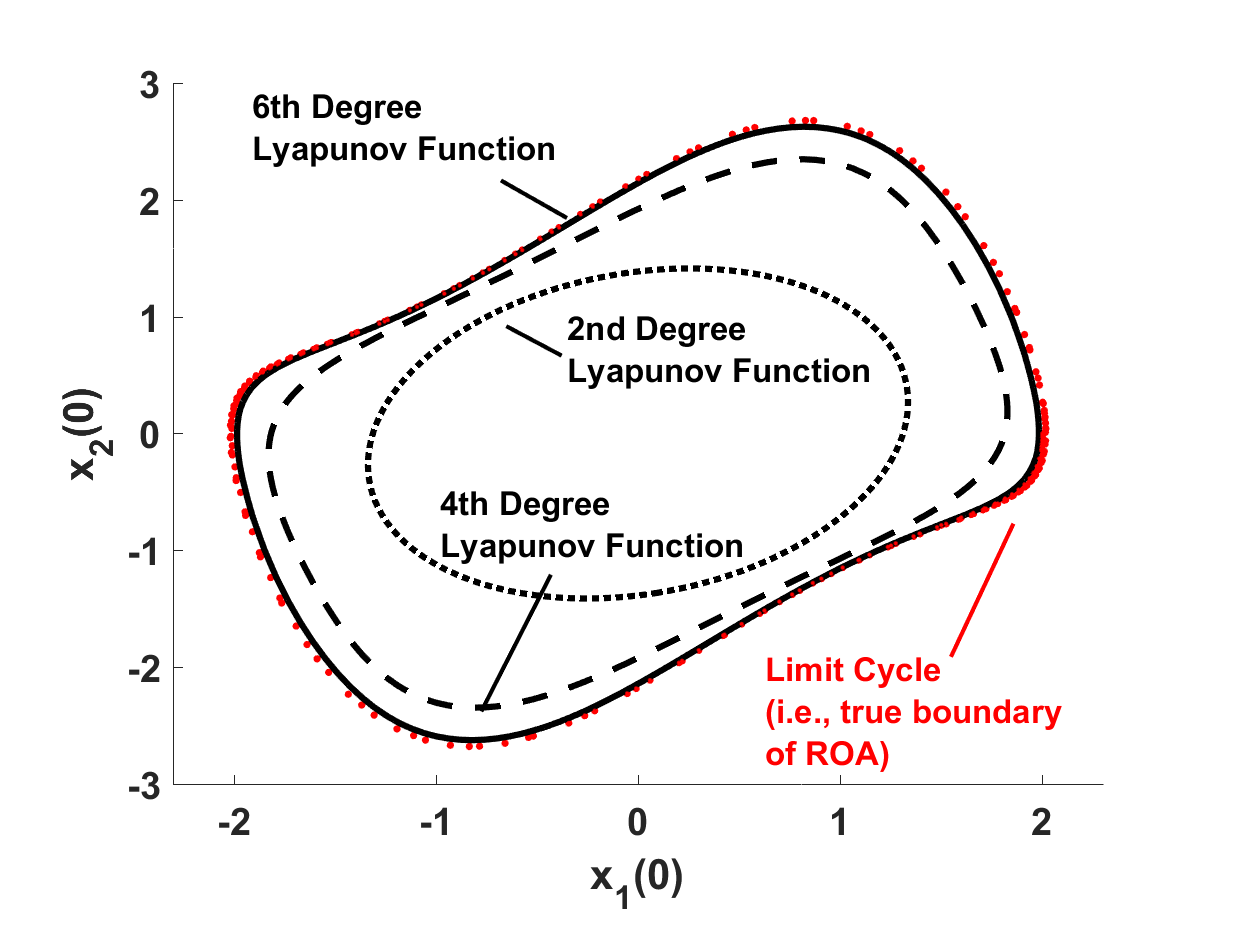
\includegraphics[width=0.65\columnwidth]{figures/my_figure.eps}
		\end{center}
		\item Note that you can nest the figure within ordered lists too
	\end{itemize}
\end{frame}


%%%%%%%%%%%%%%%%%%%%%%%%%%%%%% Slide %%%%%%%%%%%%%%%%%%%%%%%%%%
%%%%%%%%%%%%%%%%%%%%%%%%%%%%
\begin{frame}[fragile,t]{Multiple Figures}
	\begin{itemize}
		\item If you want to make multiple figures side-by-side, you can just set the sum of the figures' column widths to be $\leq 1.0$
		{\tiny
		\begin{lstlisting}
\begin{center}
	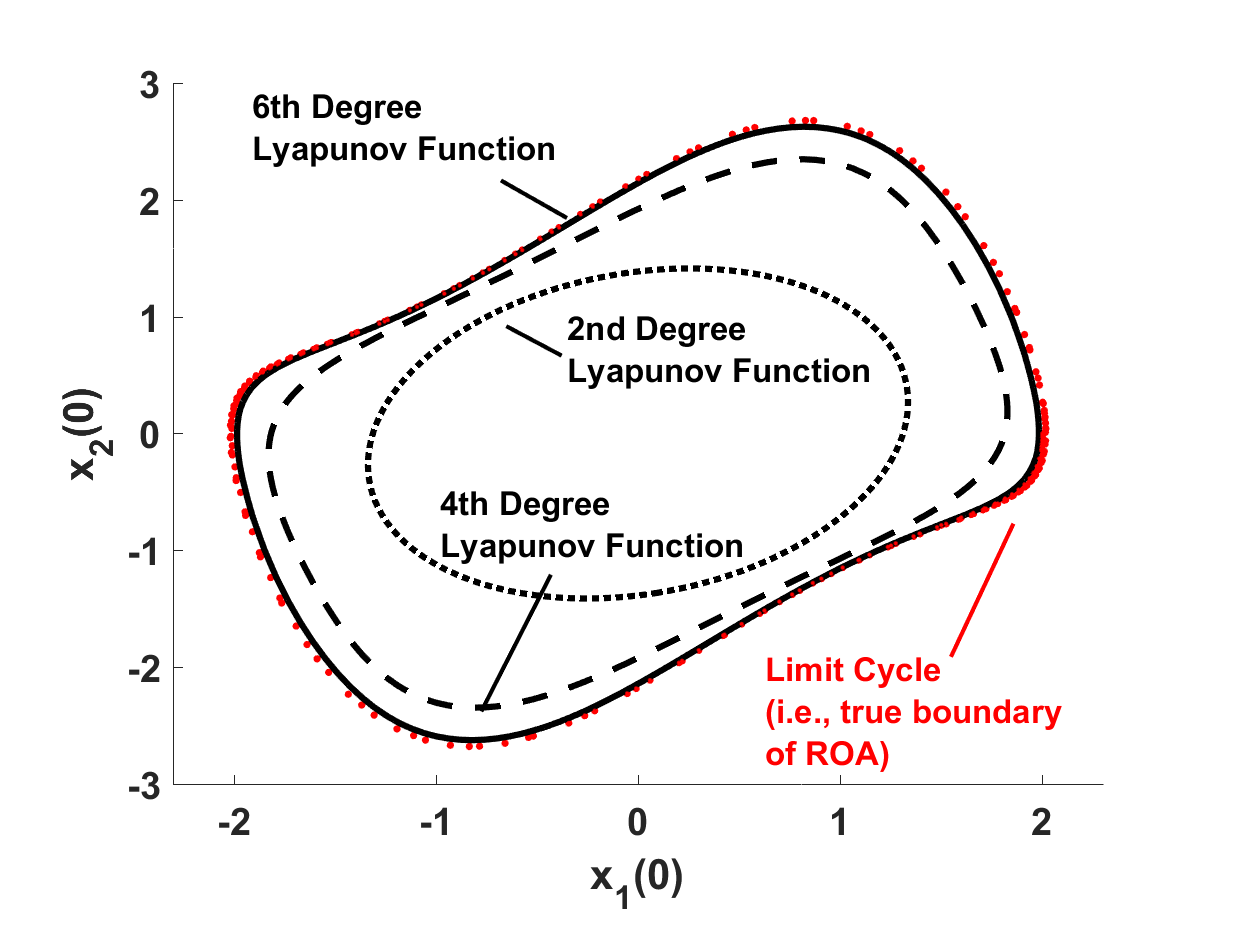
\includegraphics[width=0.35\columnwidth]{figures/my_figure.eps}
	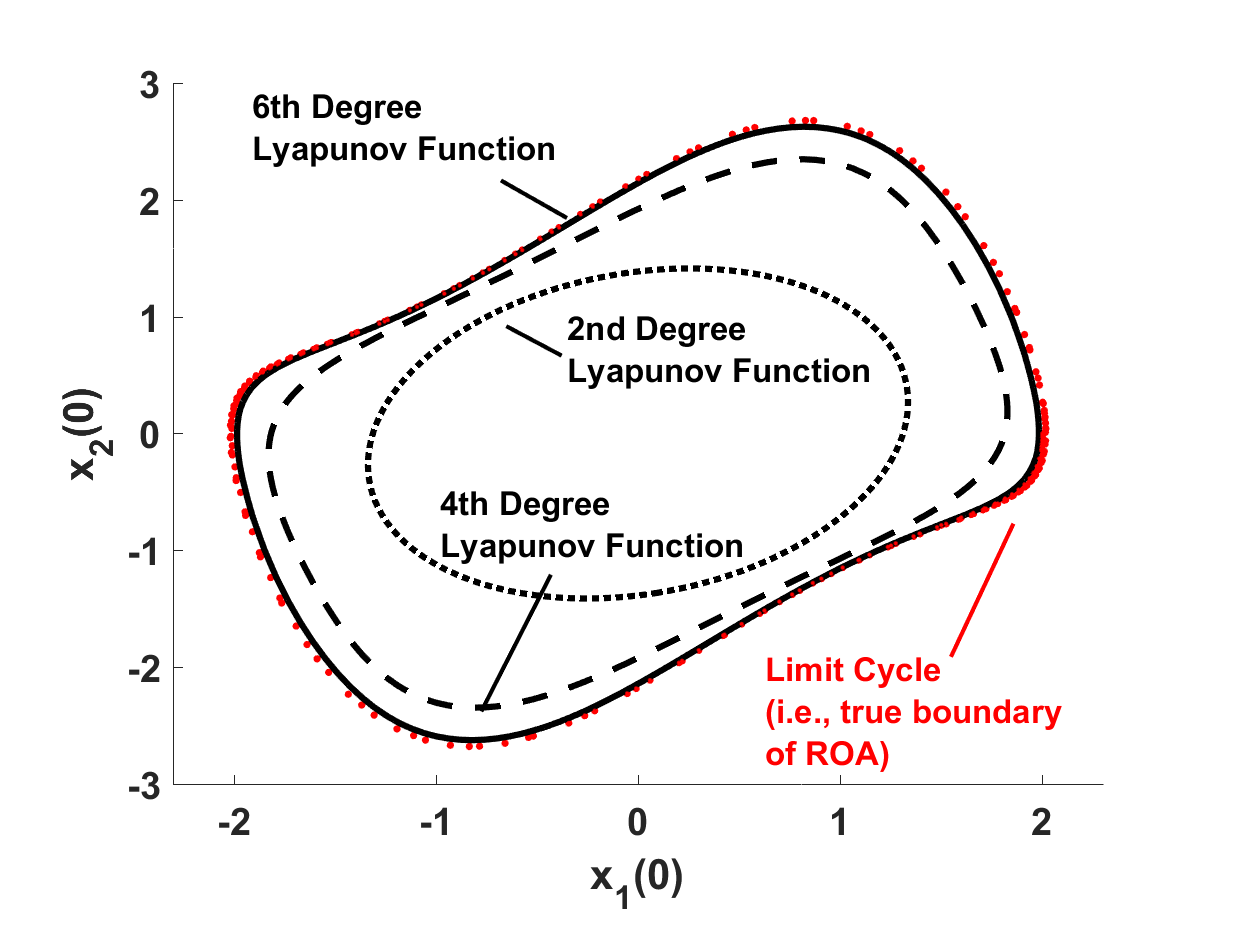
\includegraphics[width=0.45\columnwidth]{figures/my_figure.eps}
	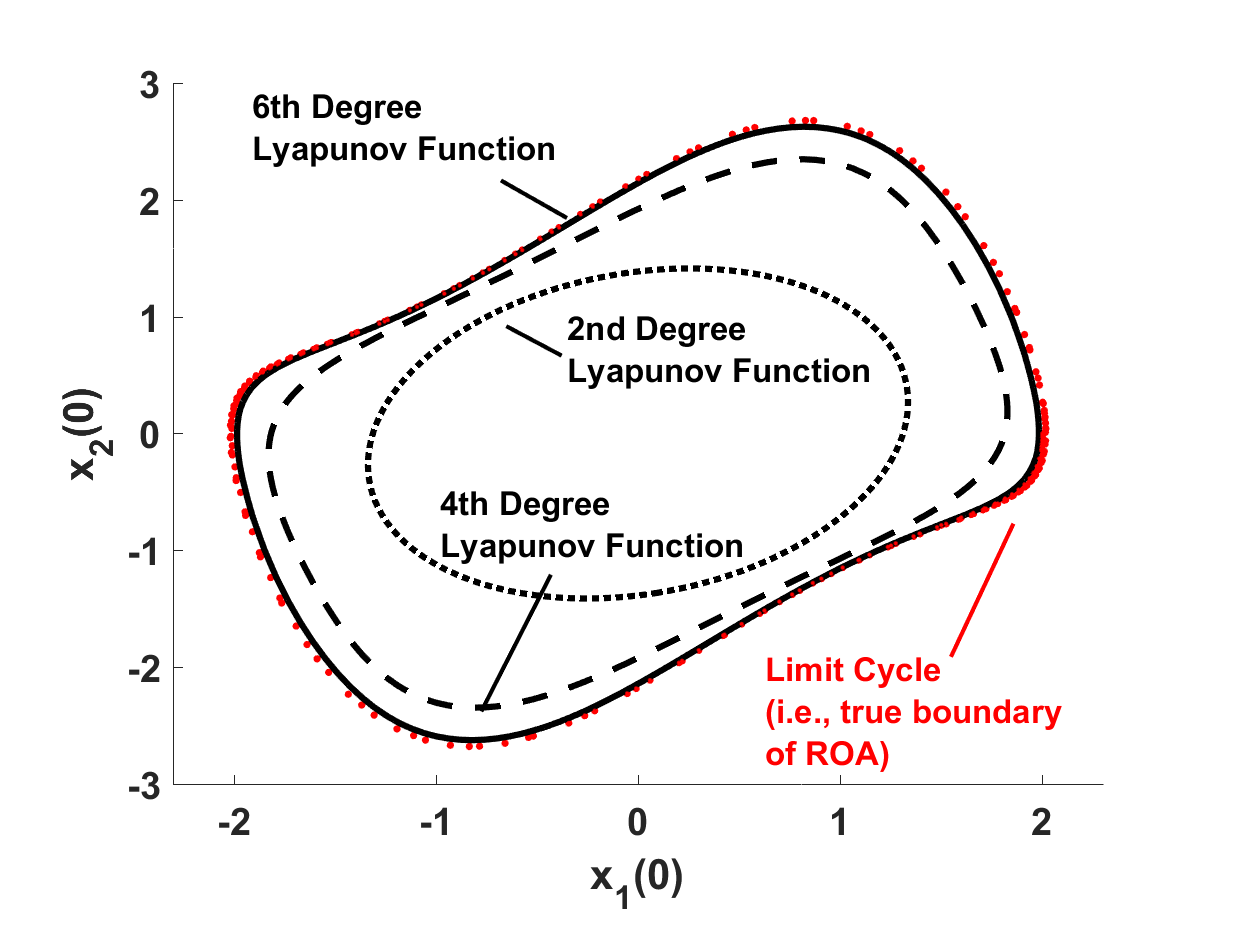
\includegraphics[width=0.15\columnwidth]{figures/my_figure.eps}
\end{center}
		\end{lstlisting}
		}
		\begin{center}
			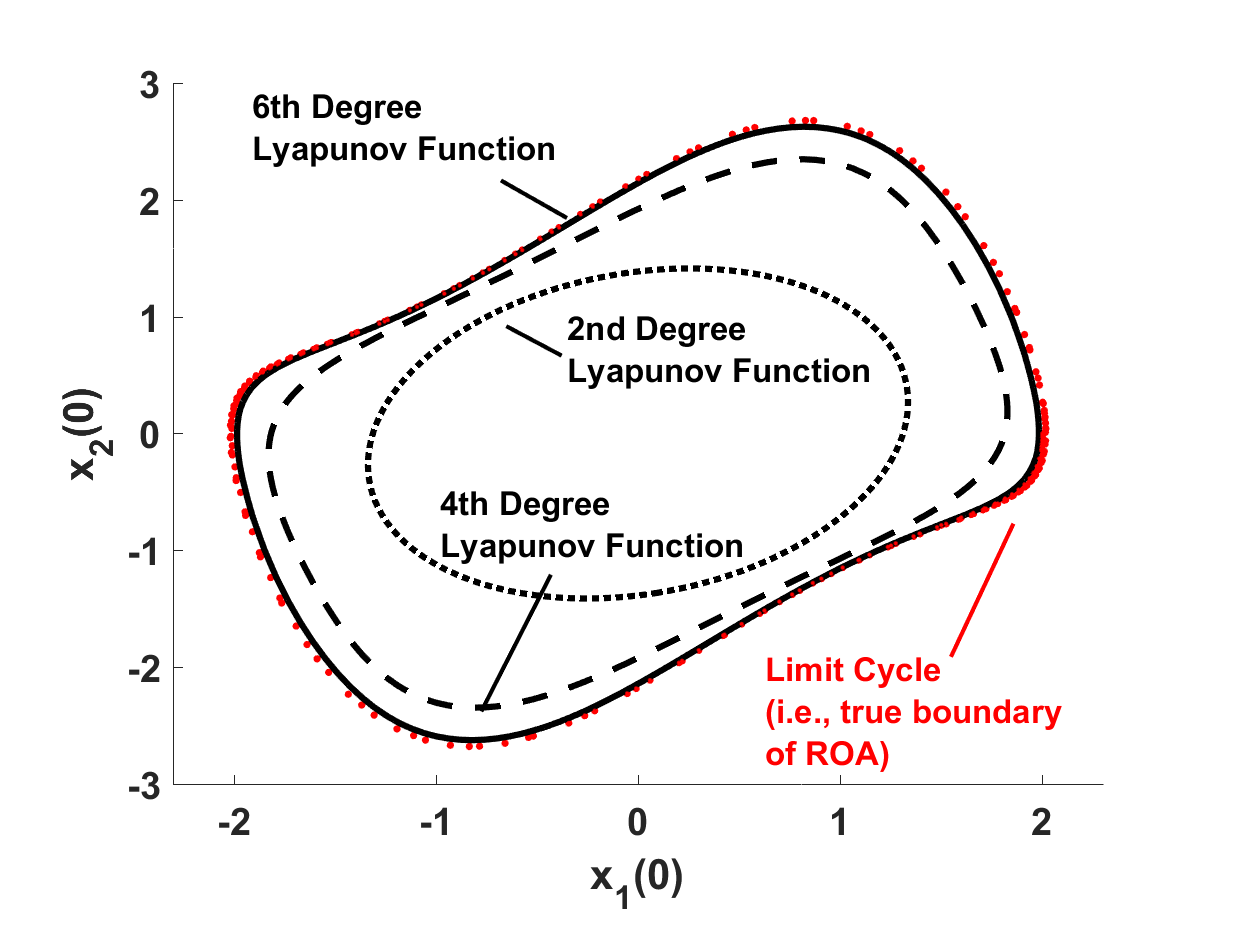
\includegraphics[width=0.35\columnwidth]{figures/my_figure.eps}
			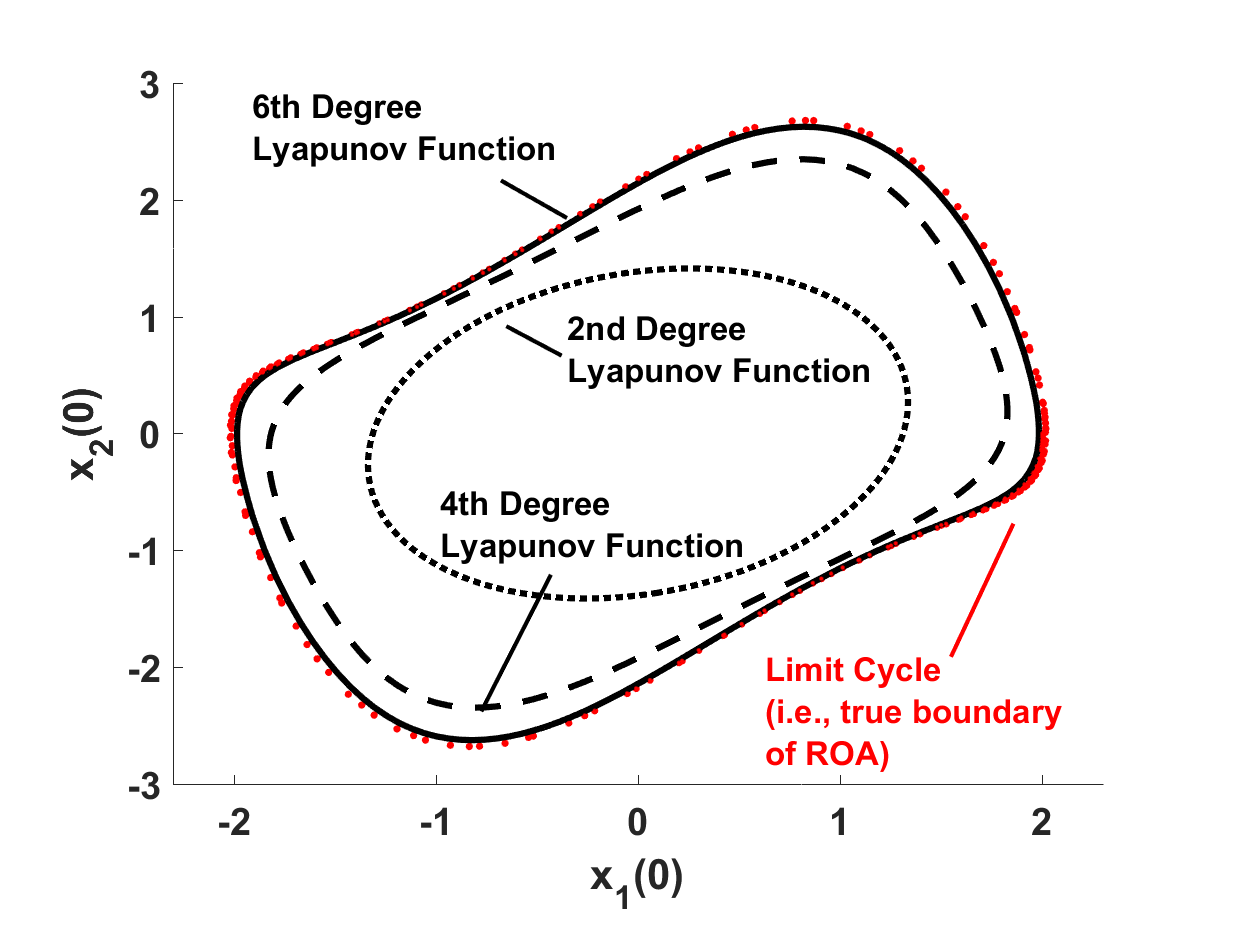
\includegraphics[width=0.45\columnwidth]{figures/my_figure.eps}
			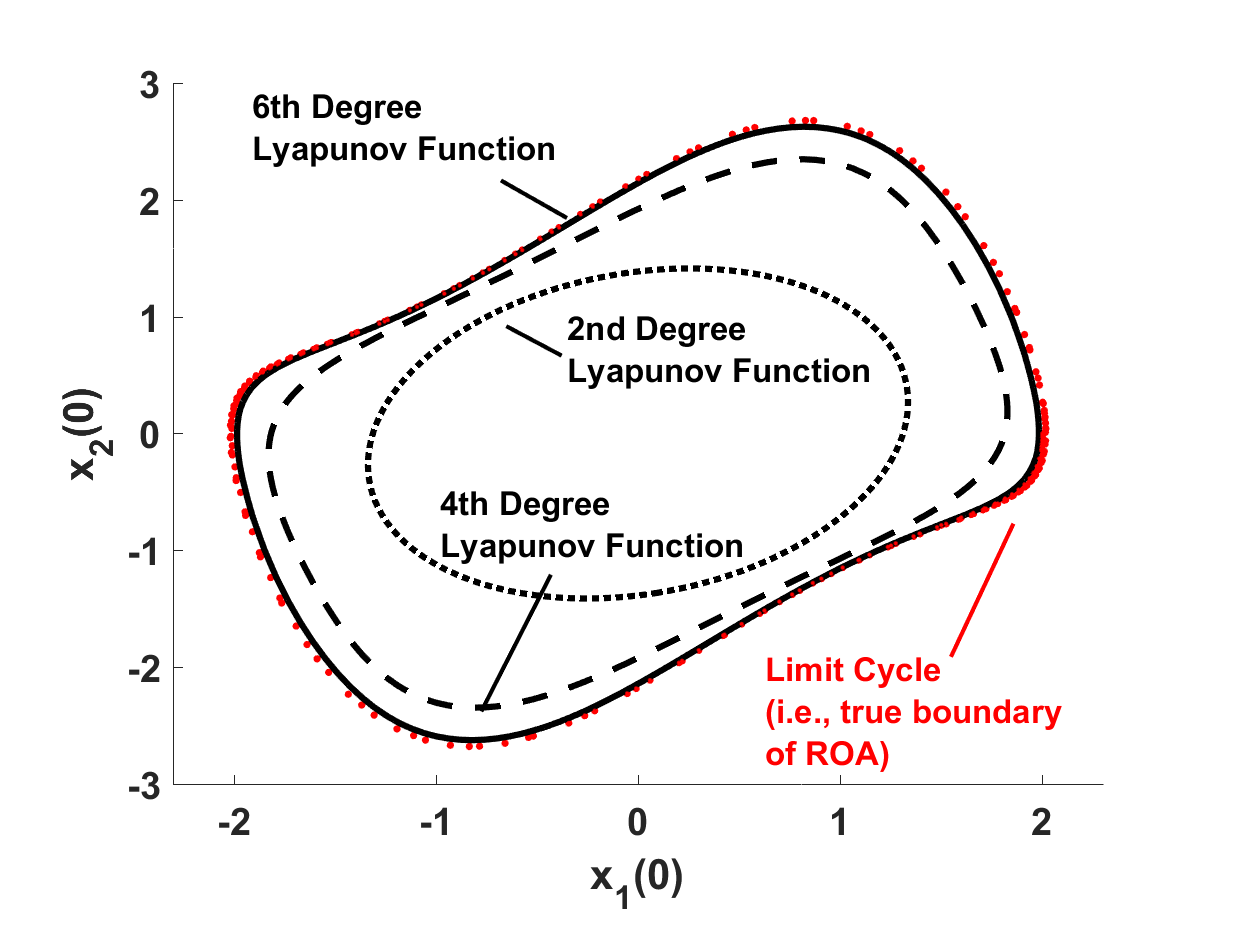
\includegraphics[width=0.15\columnwidth]{figures/my_figure.eps}
		\end{center}
		\item If the sum is $> 1.0$ then it will stack them vertically
	\end{itemize}
\end{frame}
